\documentclass{article} % EXPAND THE PREAMBLE TO SEE ALL OF THE CODE
\usepackage[utf8]{inputenc}
\usepackage{amsmath, amsfonts} 
\allowdisplaybreaks
\usepackage{amssymb}
\usepackage{esint} % for more integral symbols
\usepackage[margin=1.75in]{geometry} % [margin=1.0in]
\usepackage{graphicx} % more arguments for the \includegraphics command
\usepackage{wrapfig} 
\usepackage{textcomp} % more text symbols
\usepackage{mwe} % used for idk?
\usepackage{gensymb} % for symbols (e.g \degree and \ohm)
\providecommand{\e}[1]{\ensuremath{\times 10^{#1}}}
\usepackage{multicol} % for columns
\usepackage{float} % to better format tables
\restylefloat{table} % to better format tables
\usepackage{tabularx} % to better format tables
\usepackage{titlesec} 
\usepackage{enumitem} % allows better formatting for list environments
\usepackage{tikz} % graphs and drawings
\newcommand{\comment}[1]{} % for multiline comments
\usepackage[stretch=10]{microtype} % best package ever
\usepackage{booktabs} % for all your fancy table needs
\usepackage{environ}
\usepackage{siunitx}
\usepackage{mathrsfs}
\usepackage{cancel}
\usepackage{multirow} % allows multirow cells in tables
\usepackage{xcolor} % fancier color options
\usepackage{tikz-qtree} % trees
\usepackage{forest} % more trees (better imo)
\usepackage{mathtools}
\usepackage{hyperref}

\usepackage{contour}
\usepackage{ulem}
\renewcommand{\ULdepth}{1.8pt}
\contourlength{0.8pt}

\newcommand{\myuline}[1]{
  \uline{\phantom{#1}}%
  \llap{\contour{white}{#1}}%
}



\renewcommand{\arraystretch}{1} 

\title{CS 451 Final Project: Formula One Database}
\author{Zane Globus-O'Harra}
\date{\textit{23 March 2023}}

\begin{document}
\maketitle
\thispagestyle{empty}

\tableofcontents
\thispagestyle{empty}
\vspace{1.5cm}

\noindent
NOTE: All links in this PDF should be clickable.
\newpage

\pagenumbering{arabic}

\section{Cover Page}

\begin{itemize}
    \item \textbf{Author:} Zane Globus-O'Harra
    
    \item \textbf{Project Title:} Formula One Database

    \item \textbf{Connection Information:}
    \begin{itemize}
        \item \textbf{Port Number:} \texttt{3372}

        \item \textbf{Host Name:} \texttt{ix.cs.uoregon.edu}

        \item \textbf{Guest Account Login \& Password:} 

        login: \texttt{guest}

        password: \texttt{guest}

        \item \textbf{Database Name:} \texttt{f1db}

    \end{itemize}

    \item \textbf{Project URL:}
    \href{https://ix.cs.uoregon.edu/~zfg/f1db/main.html}{\texttt{https://ix.cs.uoregon.edu/\~{}zfg/f1db/main.html}}

    \item \textbf{Highlights:}
    \begin{itemize}
        \item Population of the result table (440 rows).
        \begin{itemize}
            \item The population of all tables except for the season
            table (1 row) and team table (10 rows) have at least 20 rows.
        \end{itemize}

        \item 8 applications:
        \begin{itemize}
            \item 6 applications to display driver and team results in
            different and meaningful ways.

            \item 1 application to display race information
            \textit{without} driver or team results (i.e., race name, circuit
            name, race length, number of laps, etc.).

            \item 1 application to compare the drivers of a team.
        \end{itemize}
    \end{itemize}
\end{itemize}

\section{Summary}

\subsection{High Level Overview}
The world that will be modeled will be a simplified version of a Formula
One (Formula 1, or F1) car-racing season. This will include the drivers, the teams the
drivers are in, the races, and the results of those races. 

\subsection{Kinds of Data}
The kinds of data that will be stored will be about the drivers, the
teams, and the results that those drivers receive in the races that they
participate in. I'm not sure how in-depth you want me to go when
discussing kinds of data, but I think that the high level overview and
the ER diagram in the Logical Design section make it fairly clear the
kinds of data that I will be keeping track of. 

\subsection{Application Programs}
The application programs that are desired are a way to summarize the
results in a season, and determine who was the champion for that season.
I also want to look at the average results of each driver, and give a
summary of their best and worst races in a season (if I add data for
multiple seasons, then I will also be able to look at their results
across their career).

Each team will have two drivers, and I will have a way to compare the
drivers of one team. I will also have a way to look at the results of a
team over a season (the team's results is the sum of the results of its
drivers), and the results of that team over its tenure in F1.


\section{Logical Design}

\begin{figure}[H]
    \centering
    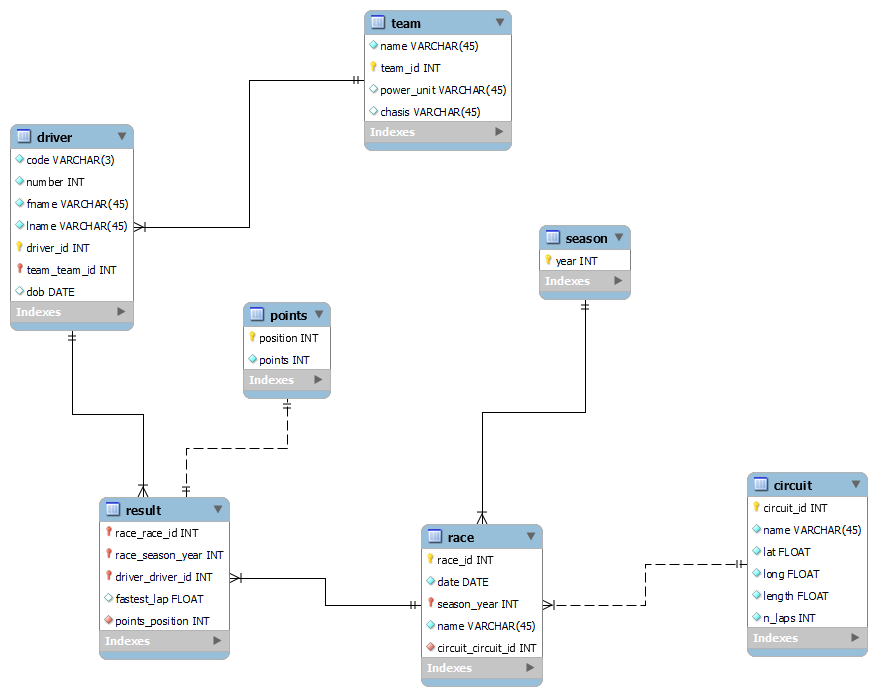
\includegraphics[scale=0.4]{f1db.png}
\end{figure}

\section{Physical Design}

Table names are in \textbf{bold and CAPITALIZED}, primary keys are
\myuline{underlined}, and foreign keys are \textit{italicized}. If an
attribute is a primary key and a foreign key, then it is
\myuline{\textit{underlined and italicized}}. Not
null requirements are indicated. Primary keys and foreign keys are
always not null.

\begin{itemize}
    \item \textbf{TEAM}: \myuline{team\_id}, name, power\_unit, chasis
    \begin{itemize}
        \item not null: power\_unit, chasis

    \end{itemize}

    \item \textbf{DRIVER}: \myuline{driver\_id},
    \textit{team\_team\_id}, code, number, fname, lname, dob
    \begin{itemize}
        \item not null: code, number, fname, lname

        \item \textit{team\_team\_id} references \textbf{TEAM}

    \end{itemize}

    \item \textbf{RESULT}: \myuline{\textit{race\_race\_id}},
    \myuline{\textit{race\_season\_year}}, \myuline{\textit{driver\_driver\_id}},
    \textit{points\_position}, fastest\_lap
    \begin{itemize}
        \item \myuline{\textit{race\_race\_id}} references \textbf{RACE}

        \item \myuline{\textit{race\_season\_year}} references
        \textbf{SEASON} 

        \item \myuline{\textit{driver\_driver\_id}} references
        \textbf{DRIVER} 

        \item \textit{points\_position} references \textbf{POINTS}
    \end{itemize}

    \item \textbf{POINTS}: \myuline{position}, points
    \begin{itemize}
        \item not null: points
    \end{itemize}

    \item \textbf{RACE}: \myuline{race\_id},
    \myuline{\textit{season\_year}}, \textit{circuit\_circuit\_id},
    date, name 
    \begin{itemize}
        \item not null: date, name

        \item \myuline{\textit{season\_year}} references \textbf{SEASON}

        \item \textit{circuit\_circuit\_id} references \textbf{CIRCUIT}
    \end{itemize}

    \item \textbf{SEASON}: \myuline{year}

    \item \textbf{CIRCUIT}: \myuline{circuit\_id}, name, lat, long,
    length, n\_laps
    \begin{itemize}
        \item not null: name, lat, long, length, n\_laps
    \end{itemize}
\end{itemize}


\section{List of Applications}

\begin{enumerate}[label=(\arabic*)]
    \item % season_driver_results.php -- DONE
    input: season

    output: summary of the all driver's results across that season

    \item % season_team_results.php -- DONE
    input: season

    output: summary of the team (constructor) results of that season

    \item % race_driver_res.php -- DONE
    input: race, season 
    
    output: summary of the driver's results from that one race in that season

    \item % race_team_res.php -- DONE
    input: race, season 
    
    output: summary of the team's results from that race in that season

    \item % driver_season_res.php -- DONE
    input: driver, season

    output: A single driver's race results across that season 

    \item % driver_avg_season.php -- DONE
    input: driver, season

    output: average results of that driver across that season

    \item % season_race_info.php -- DONE
    input: season

    output: summary of the races in that season (race name, circuit
    name, circuit length, number of laps, etc.)

    \item % team_driver_cmp_season.php -- DONE
    input: team, season 

    output: for each race in that season, compare the results of the
    drivers in that team

\end{enumerate}


\section{User's Guide}

\subsection{Basic Overview}

Each ``application'' is fairly straightforward to use. Most of the
applications display some variation of the results over a season.
Seasons are determined by the year, and the only season that has data is
2021. However, the complete data for every race and every result has
been entered for the 2021 F1 season, so every query for that season
should return a fairly ``well-stocked'' set of results.

The other fields are fairly picky about what is entered. If a field asks
for a ``Race,'' it wants that race's full name. The available races are:
\begin{multicols}{2}
\begin{itemize}
    \itemsep-0.1em
    \item Bahrain Grand Prix
    \item Emilia Romagna Grand Prix
    \item Portugese Grand Prix
    \item Spanish Grand Prix
    \item Monaco Grand Prix
    \item Azerbaijan Grand Prix
    \item French Grand Prix
    \item Styrian Grand Prix
    \item Austrian Grand Prix
    \item British Grand Prix
    \item Hungarian Grand Prix
    \item Belgian Grand Prix
    \item Dutch Grand Prix
    \item Italian Grand Prix
    \item Russian Grand Prix
    \item Turkish Grand Prix
    \item United States Grand Prix
    \item Mexico City Grand Prix
    \item Sao Paulo Grand Prix
    \item Qatar Grand Prix
    \item Saudi Arabian Grand Prix
    \item Abu Dhabi Grand Prix
\end{itemize}
\end{multicols}

The same goes for drivers, whose last names are:
\begin{multicols}{2}
\begin{itemize}
    \itemsep-0.1em
    \item Raikkonen
    \item Giovinazzi
    \item Gasly
    \item Tsunoda
    \item Alonso
    \item Ocon
    \item Vettel
    \item Stroll
    \item Leclerc
    \item Sainz
    \item Mazepin
    \item Schumacher
    \item Ricciardo
    \item Norris
    \item Hamilton
    \item Bottas
    \item Perez
    \item Verstappen
    \item Latifi
    \item Russell
    \item Kubica
\end{itemize}
\end{multicols}

And lastly, the same goes for the teams:

\begin{multicols}{2}
\begin{itemize}
    \itemsep-0.1em
    \item Mercedes-AMG Petronas F1 Team
    \item Red Bull Racing Honda
    \item Scuderia Ferrari
    \item McLaren F1 Team
    \item Aston Martin Cognizant F1 Team
    \item Alpine F1 Team
    \item Alfa Romeo Racing Orlen
    \item Scuderia AlphaTauri Honda
    \item Haas F1 Team
    \item Williams Racing
\end{itemize}
\end{multicols}

\subsection{Examples of Each Application}

Examples for each app are as follows:
\begin{figure}[H]
    \centering
    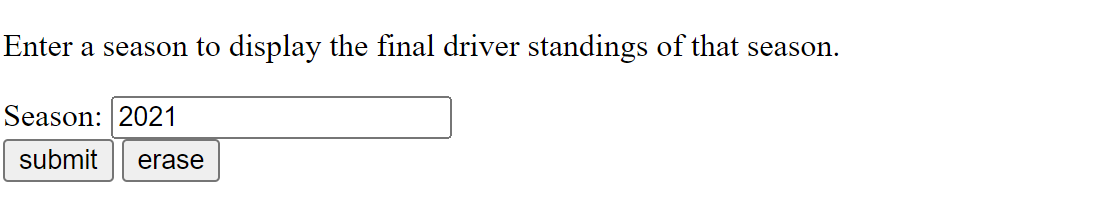
\includegraphics[scale=0.35]{1.PNG}
    \caption{This app displays the final driver standings of a season,
    by summing up the points that each driver has earned over the season
    and ordering the drivers based on total points earned.}
\end{figure}

\begin{figure}[H]
    \centering
    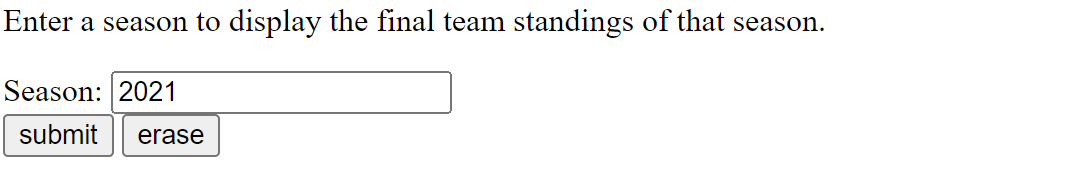
\includegraphics[scale=0.35]{2.PNG}
    \caption{This app displays the final team standings of a season,
    by summing up the points that each team has earned over the season
    and ordering the team based on total points earned. Because each
    team has two drivers, the points that a team earns in a race is the
    sum of the points of the drivers of that team.}
\end{figure}
\begin{figure}[H]
    \centering
    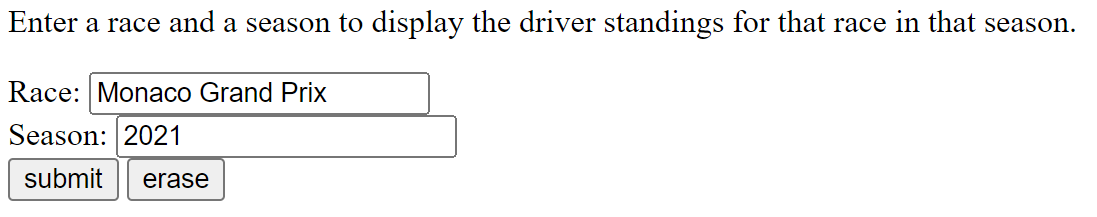
\includegraphics[scale=0.35]{3.PNG}
    \caption{This app displays the driver standings after a race,
    showing their name, the position they finished in, and the points
    that they earned.}
\end{figure}
\begin{figure}[H]
    \centering
    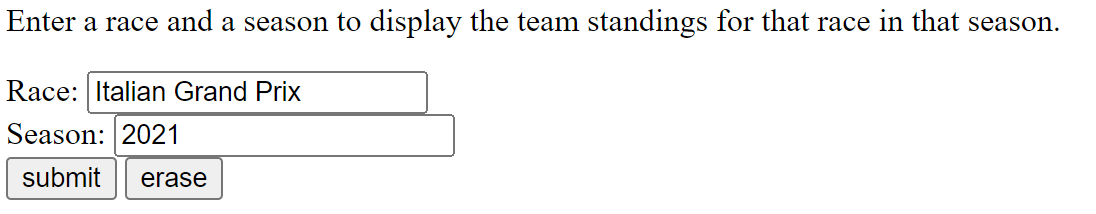
\includegraphics[scale=0.35]{4.PNG}
    \caption{This app displays the team standings after a race,
    showing their name, the position they finished in, and the points
    that they earned. The teams finishing position is determined by the
    points that the drivers of that team earned.}
\end{figure}
\begin{figure}[H]
    \centering
    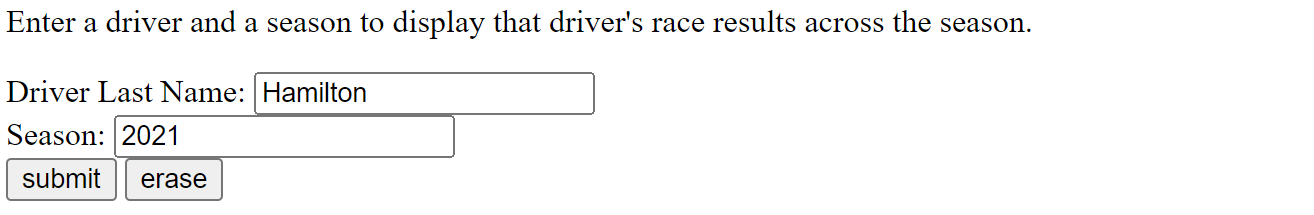
\includegraphics[scale=0.35]{5.PNG}
    \caption{This app displays, in chronological order across a season,
    the race results of one driver as well as the points that that
    driver earned.}
\end{figure}
\begin{figure}[H]
    \centering
    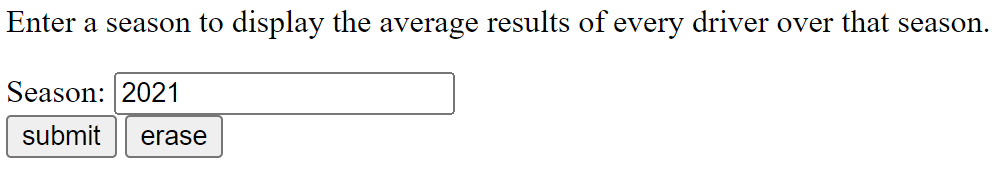
\includegraphics[scale=0.35]{6.PNG}
    \caption{This app displays the average position per race and average
    points per race for every driver in a season, ordered from the highest
    average points to the lowest.}
\end{figure}
\begin{figure}[H]
    \centering
    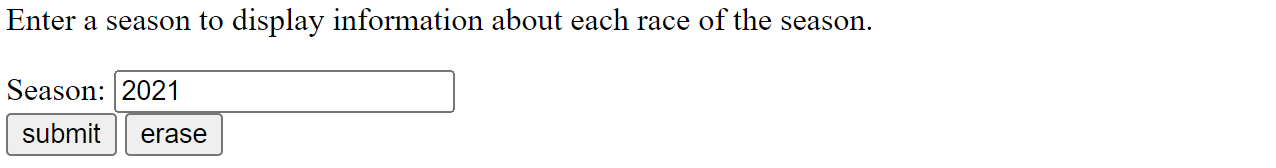
\includegraphics[scale=0.35]{7.PNG}
    \caption{This app displays information about every race that occurs
    in a season, including the race name, the circuit at which the race
    takes place, the date of the race, the length of the circuit, the
    number of laps, and the total length of the race. The results are
    ordered chronologically by race date.}
\end{figure}
\begin{figure}[H]
    \centering
    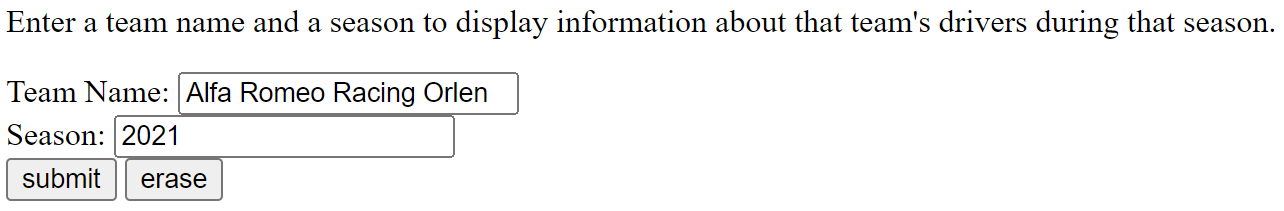
\includegraphics[scale=0.35]{8.PNG}
    \caption{This app displays the two drivers in a team, mainly to
    compare the number of points that each driver has earned, but also
    showing their driver codes, their number, and the number of races
    they have completed. The drivers' ages are also displayed, and it
    should be noted that these are \textit{not} the drivers' current ages,
    rather they are the drivers' ages during the specified season. If a
    needed a replacement driver for some races during the season, that
    is displayed here (as is the case with Alfa Romeo).}
\end{figure}


\section{Contents of the Tables}

The contents of the tables can be found by clicking on the link to the
table contents from the main project URL, or by going directly to:

\noindent
\href{https://ix.cs.uoregon.edu/~zfg/f1db/tables.html}{\texttt{https://ix.cs.uoregon.edu/\~{}zfg/f1db/tables.html}}

\section{Implementation Code}

The implementation code for the main website can be found via a link at
the bottom of the main project webpage. The code for each PHP app can be
found via a link below each submission form. The link to the main
website is repeated here:

\noindent
\href{https://ix.cs.uoregon.edu/~zfg/f1db/main.html}{\texttt{https://ix.cs.uoregon.edu/\~{}zfg/f1db/main.html}}


\section{Conclusion}

\subsection{Reflection About the Project}

Looking back on what I have done in this project, I would say that the
bulk of the work was split into three parts:
\begin{enumerate}[label=(\arabic*)]
    \item Designing the database.
    \item Entering data.
    \item Creating the applications.
\end{enumerate}

After creating my initial Chen diagram for part 1 of this project, I
revised it and updated it for part 2 into a Crowsfoot diagram made in
MySQL workbench so that I could easily turn the ER diagram into an
actual database with tables. This part took a while because of the
planning and thinking that was involved around how to organize the data,
as well as what data I needed for the applications that I wanted to
make.
\medskip

Once I had the design that I wanted, I then needed to enter the data. I
decided to enter the data for one entire Formula 1 season. While I could
have easily used the more recent 2022 season data, I decided to instead
use the 2021 season data because that was a very exciting season with
many thrilling races. The data that I used was from
Wikipedia,\footnote{The data was mainly from 
\href{https://en.wikipedia.org/wiki/2021_Formula_One_World_Championship}
{\texttt{wikipedia.org/wiki/2021\_Formula\_One\_World\_Championship}},
as well as the Wikipedia pages associated with each driver, race, and
circuit.} and I could find no easy way to enter it in bulk (I'm sure if
I searched harder I could have found a way, but oh well), so I entered
it all manually. For the most part this wasn't too tedious, except for
the results table, which was 440 rows.
\medskip

Once I had the data entered, I set about creating the applications. I
already had an idea about what applications I wanted to make (my
original application ideas are still listed in section 2.3), so I
started with those ideas. Because I only had the data for one season,
this meant that I couldn't compare a driver's results across seasons, so
I had to change some of my applications to account for this.
Additionally, I found it exceptionally difficult to create a query that
would tell me the best and worst results of a driver, so I ended up
abandoning that. 

Instead, I added applications to display information about each race of
a season, as well as some additional ways to display the results of each
driver or team on a per race or per season basis.
\medskip

I also want to add some of my reasoning behind adding an ID field to
many of the tables. While drivers could have been ID'd by their code, if
I had added previous seasons, then there would be an overlap between the
driver code of ``MSC'' for Mick Schumacher and his father, Michael
Schumacher, who also raced in F1. There is similar reasoning for the
other tables (e.g., races change names depending on the season, and so
do the teams' names, and so on).

\subsection{Simplifications}

While my database captures a great deal of the scoring system and
results system of Formula 1, it has nevertheless been simplified. Some
things that my database simplifies are:
\begin{itemize}
    \item Tiebreakers: When two drivers have the same score at the end
    of a season, their race results are ``counted back,'' and the driver
    with higher ranking finishes wins the tie. There is no such thing in
    my database, and ties are broken by the alphabetical order of
    drivers' names.

    \item Fastest laps: When a driver finishes a race in the top 10 and
    has completed the fastest lap in that race, they earn an additional
    point. My database includes no such rule.

    \item Partially awarded points: When a race does not complete the
    full race distance, half points are awarded. This occurred in the
    2021 Belgian Grand Prix due to poor weather conditions. My database
    does not have a rule to allow this.
    
    \item Sprint races: I won't go into the details of what a sprint
    race entails, but it adds another layer of complexity to the point
    system. 

    \item Qualifying: A qualifying session precedes every race to
    determine the order of the starting grid. Ideally my database would
    include the results of this qualifying session as well, because then
    I could create a query that could examine the positions gained or
    lost in the race relative to a driver's starting position.
\end{itemize}
The list goes on, but these are the main areas that my database has
simplified. 

\subsection{Things I Would Have Done Differently}

Aside from the simplifications mentioned in section 9.2, I would have
done two main things differently:
\begin{itemize}
    \item Change fastest laps: As they currently are, fastest laps have
    only one column and they are in units of minutes. I think that it
    would have been better to split fastest lap into two columns, one
    for the minutes and one for the seconds. While none of my
    applications involved fastest laps, I think that this would have
    made queries involving fastest laps easier to write (i.e., I
    wouldn't have to convert 1.5 minutes to 1 minute and 30 seconds
    because it would already be in the minute-second format).

    \item Have an additional table for engines: In the team table, I
    have the engine that each team uses as a column. However, some teams
    buy engines from other teams, and thus use the same engine (e.g.,
    Mercedes-AMG Petronas F1 Team produces the Mercedes-AMG F1 M12
    engine, which is also used by Mclaren F1 Team, Aston Martin
    Cognizant F1 Team, and Williams Racing). This violates the ``one
    fact in one place'' motto.

    \item Have a better system for calculating a team's position results 
    based on one race. As it is, I use the \texttt{RANK() OVER} function
    in MySQL, which ranks each team based on the sum of the points that
    the drivers earned in a race. However, if two teams earned the same
    number of points, then their position is the same. This does not
    adhere to real life, where driver positions come into play when
    teams have the same number of points. I would have liked to
    implement this, but there were a great deal of rules that are
    tricky, and I was struggling to get everything figured out. So
    instead I used a simplified version.
\end{itemize}
Other than those two small changes, I am quite happy with how this
project turned out, and I think that despite being somewhat simple, my
database does a fairly good job at modeling a Formula 1 season.



\end{document}
